\providecommand{\main}{../..}
\documentclass[\main/thesis.tex]{subfiles}
\begin{document}

\section{The Next Numeral}\label{next}

Paul Benacerraf once argued\cite{benacerraf1965numbers} that, there are two kinds
of \textit{counting} which correspond to \textbf{transitive} and \textbf{intransitive}
uses of the verb ``to count.'' Transitive counting, in his sense, is to assign one
of the numbers to the cardinality of a set, by establishing a one-to-one correspondence
between the numbers and the objects one is counting, all the way from none to
all. Intransitive counting, on the other hand, is to generate a sequence of
notation, that could go as far as we need. And it seems that one can only learn
how to count intransitively first, before knowning how to count transitively,
but not vice versa. So it is important to know how to generate the next numeral
we need.

\subsection{Definition}

There are countably infinite numerals in most systems (of $ d \textgreater 0 $)
and we can always find a sequence to enumerate them from {\lstinline|zero ∙|} to
any notation.
Although these enumerations are isomorphic to natural numbers, that is not how we
count with these numerals. Instead, we evaluate these numerals to natural numbers
in a way we see fit. As a result, the evaluation may not be surjective, which
causes the line segment to be gapped      .

\begin{center}
    \begin{adjustbox}{max width=\textwidth}
        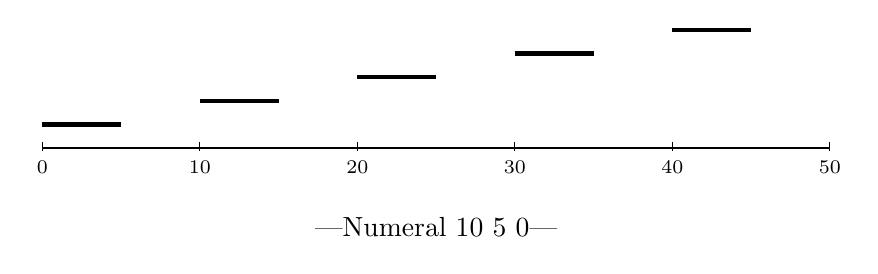
\begin{tikzpicture}
            % a straight line segment
            \draw (0, 0) -- (10, 0);
            % the ticks and their labels
            \foreach \x  in {0,...,5}
                \draw[xshift=\x*2 cm] (0pt,2pt) -- (0pt,-1pt) node[below,fill=white] {\scriptsize\the\numexpr\x*10\relax};
            \foreach \x  in {0,...,4}
                \draw[ultra thick, xshift=\x*2 cm, yshift=\x*0.3 cm] (0,0.3) -- (1,0.3);
            % labels
            \node at (5, -1) {{\lstinline|Numeral 10 5 0|}};
        \end{tikzpicture}
    \end{adjustbox}
\end{center}
\begin{center}
    \begin{adjustbox}{max width=\textwidth}
        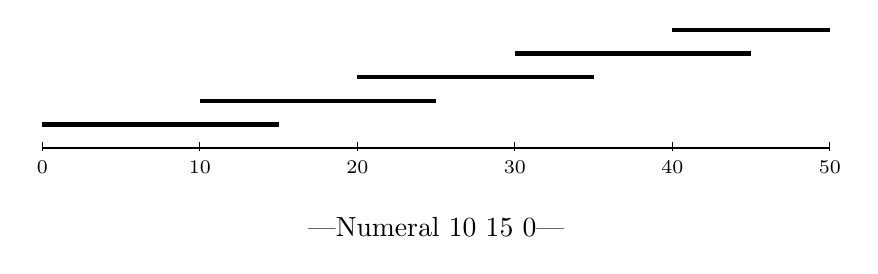
\begin{tikzpicture}
            % a straight line segment
            \draw (0, 0) -- (10, 0);
            % the ticks and their labels
            \foreach \x  in {0,...,5}
                \draw[xshift=\x*2 cm] (0pt,2pt) -- (0pt,-1pt) node[below,fill=white] {\scriptsize\the\numexpr\x*10\relax};
            \foreach \x  in {0,...,3}
                \draw[ultra thick, xshift=\x*2 cm, yshift=\x*0.3 cm] (0,0.3) -- (3,0.3);
            \draw[ultra thick, xshift=8 cm, yshift=1.2 cm] (0,0.3) -- (2,0.3);
            % labels
            \node at (5, -1) {{\lstinline|Numeral 10 15 0|}};
        \end{tikzpicture}
    \end{adjustbox}
\end{center}

% However, these sequences of enumeration are not the


{\lstinline|b|}.
% Among those countably infinitely many numerals,
%
% we can enumerate
% their countably infinitely many numerals in an unambigouos way.

% In natural numbers à la Peano, finding the next number is as simple as placing
% a counting rod. The syntax aligns perfectly with the semantics (or we can argue
% that the syntax itself is the semantics we are persuing)
% , nothing can go wrong.


% In natural numbers, the successor also happens to be the next number.
% However, things are not so simple in our representation.

%
%
% Given a numeral that is not a maximum, find the next.

\begin{lstlisting}
next-number : ∀ {b d o}
    → (xs : Numeral b d o)
    → ¬ (Maximum xs)
    → Numeral b d o
next-number {b} {d} {o} xs ¬max with numView b d o
next-number xs ¬max | NullBase d o = ?
next-number xs ¬max | NoDigits b o = NoDigits-explode xs
next-number xs ¬max | AllZeros b   = contradiction (Maximum-AllZeros xs) ¬max
next-number xs ¬max | Proper b d o proper = ?
\end{lstlisting}


\end{document}
